\chapter{Ecosistemas y estructura trófica}\label{ch:b1:ecosystem-organization}

Un manantial de una llanura caliza vierte un agua tan clara que cada planta,
cada pez y cada tortuga que hay en ella pueden contarse desde una barca. La
luz del sol cae sobre las cintas acuáticas a razón de \qty{1.7}{} millones
de kilocalorías por metro cuadrado y año; las plantas almacenan el uno por
ciento; los caracoles y las tortugas que las comen obtienen una sexta parte
de eso; los peces que comen caracoles, una décima parte más; y la única
garza que hay en lo alto vive de la cienmilésima parte de lo que cayó sobre
el agua. Todos los \omterm{def:b1:ecosystem-organization:ecosystem}{ecosistemas} están construidos así: una corriente de
energía que entra una vez, pasa de los comidos a los que comen y sale como
calor, mientras que la materia que mueve se recicla. Este capítulo define el
\omterm{def:b1:ecosystem-organization:ecosystem}{ecosistema} y sus partes, el \omterm{def:b1:ecosystem-organization:niche}{nicho} que ocupa cada especie, los \omterm{def:b1:ecosystem-organization:trophic}{niveles
tróficos} y las \omterm{def:b1:ecosystem-organization:foodweb}{redes alimentarias} por los que fluye la energía, la
productividad que fija el tamaño del conjunto, y las maneras de contar
cuántas clases de seres viven en él.

\section{Ecosistema y nicho}

\begin{definition}[Ecosistema, biotopo, comunidad]\label{def:b1:ecosystem-organization:ecosystem}
\index{ecosistema}\index{biotopo}\index{comunidad}
Un \emph{ecosistema} es el conjunto de \omterm{def:b1:organism-environment:organism}{organismos} que viven en un lugar
definido junto con el medio físico que ocupan y con el que intercambian: la
\emph{comunidad} (o biocenosis) --- todas las poblaciones de todas las
especies --- y el \emph{biotopo} --- el suelo, el agua, el aire, la luz y el
clima. Sus límites se eligen según la pregunta: un tronco podrido, una
charca, un bosque, una cuenca oceánica, la biosfera entera. Un ecosistema es
un \omterm{def:b1:organism-environment:organism}{sistema abierto} (\cref{ch:b1:organism-environment}): la energía lo
atraviesa, la materia circula dentro de él y a través de sus fronteras, y su
estructura es el patrón de quién come a quién.
\end{definition}

\begin{definition}[Hábitat, nicho]\label{def:b1:ecosystem-organization:niche}
\index{nicho ecológico}\index{hábitat}
El \emph{hábitat} de una especie es dónde vive; su \emph{nicho} es cómo
vive: el conjunto completo de condiciones que tolera y de recursos que usa
--- temperatura, humedad, luz, alimento, momento de actividad, lugares de
nidificación ---, cada uno de ellos una dimensión a lo largo de la cual la
especie ocupa un intervalo. El \emph{nicho fundamental} es el intervalo que
podría ocupar sola; el \emph{nicho realizado}, la parte que ocupa de hecho
en presencia de competidores y depredadores
(\cref{ch:b1:species-interactions}). Dos especies con el mismo nicho no
pueden coexistir mucho tiempo en un mismo lugar; los nichos de las especies
que coexisten difieren, y la \omterm{def:b1:ecosystem-organization:ecosystem}{comunidad} es un conjunto de nichos encajados.
\end{definition}

\begin{omfigure}
\begin{tikzpicture}[font=\footnotesize, >=Stealth, line cap=round]
  \draw[->, thick] (0,0) -- (7.4,0) node[below left] {temperatura};
  \draw[->, thick] (0,0) -- (0,5.2) node[below right, rotate=90, anchor=south east] {};
  \node[rotate=90, anchor=south] at (-0.4,2.6) {tamaño de la presa};
  \draw[thick, omDef, fill=omDef!18] (3.6,2.6) ellipse (2.8 and 1.9);
  \node[omDef!80!black, anchor=south] at (2.5,3.7) {nicho fundamental};
  \draw[thick, omThm, fill=omThm!25] (2.9,2.3) ellipse (1.6 and 1.2);
  \node[omThm!80!black] at (2.9,2.3) {nicho realizado};
  \draw[thick, omProp, fill=omProp!25, opacity=0.8] (5.6,3.4) ellipse (1.5 and 1.1);
  \node[omProp!80!black, align=center] at (5.6,3.4) {nicho del\\ competidor};
  \node[anchor=north, align=center, gray] at (3.7,-0.5) {dos de las muchas dimensiones de un nicho; el competidor excluye a la especie del solapamiento};
\end{tikzpicture}

{\small El \omterm{def:b1:ecosystem-organization:niche}{nicho} como volumen en un espacio de condiciones y recursos, del
que se dibujan dos dimensiones. El \omterm{def:b1:ecosystem-organization:niche}{nicho} fundamental es lo que una especie
podría ocupar; el \omterm{def:b1:ecosystem-organization:niche}{nicho} realizado es lo que le dejan sus competidores.}
\end{omfigure}

\begin{example}[Cinco reinitas en una misma picea]\label{ex:b1:ecosystem-organization:warblers}
Cinco especies de pequeñas reinitas insectívoras anidan en los mismos
bosques de piceas y comen los mismos insectos; observadas de cerca, cada una
busca alimento en una parte distinta del árbol --- la copa, las acículas
nuevas del exterior, las ramas medias, el tronco y las ramas bajas, el suelo
de debajo --- y a alturas y horas distintas. Su \omterm{def:b1:ecosystem-organization:niche}{hábitat} es uno; sus \omterm{def:b1:ecosystem-organization:niche}{nichos}
son cinco, y el bosque alberga cinco especies donde el alimento por sí solo
sugeriría una.
\end{example}

\section{La estructura trófica}

\begin{definition}[Productores, consumidores, descomponedores]\label{def:b1:ecosystem-organization:trophic}
\index{nivel trófico}\index{productor}\index{consumidor}\index{descomponedor}
Los \omterm{def:b1:organism-environment:organism}{organismos} de un \omterm{def:b1:ecosystem-organization:ecosystem}{ecosistema} se agrupan según lo que comen en
\emph{niveles tróficos}. Los \emph{productores} (autótrofos: plantas, algas,
cianobacterias, bacterias quimiosintéticas) fabrican materia orgánica a
partir de la inorgánica; son el primer nivel. Los \emph{consumidores} la
comen: los \emph{consumidores primarios} (herbívoros) comen productores, los
\emph{consumidores secundarios} (carnívoros) comen herbívoros, los
consumidores \emph{terciarios} comen carnívoros; los omnívoros comen en
varios niveles. Los \emph{descomponedores} (bacterias, hongos) y los
\emph{detritívoros} (lombrices, cochinillas, escarabajos peloteros) viven de
la materia muerta y de los desechos de todos los niveles, y devuelven sus
minerales al suelo y al agua para que los productores vuelvan a captarlos
--- el eslabón que cierra el ciclo de la materia.
\end{definition}

\begin{definition}[Cadena alimentaria, red alimentaria]\label{def:b1:ecosystem-organization:foodweb}
\index{cadena alimentaria}\index{red alimentaria}
Una \emph{cadena alimentaria} es una secuencia de \omterm{def:b1:organism-environment:organism}{organismos} en la que cada
uno se come al anterior: hierba, saltamontes, rana, culebra, halcón. En una
\omterm{def:b1:ecosystem-organization:ecosystem}{comunidad} real cada especie come a varias y es comida por varias, y las
cadenas se entrelazan en una \emph{red alimentaria}, cuyas flechas van del
comido al que come --- en el sentido de la energía. Las cadenas son cortas:
rara vez más de cuatro o cinco eslabones, por una razón que da el apartado
siguiente.
\end{definition}

\begin{omfigure}
\begin{tikzpicture}[font=\footnotesize, >=Stealth, line cap=round,
  sp/.style={draw, thick, rounded corners=3pt, inner sep=3pt, align=center, fill=white}]
  \node[sp, fill=omExo!20] (grass) at (1.5,0) {cintas acuáticas, algas};
  \node[sp, fill=omExo!20] (det) at (6.5,0) {detritos};
  \node[sp, fill=omProp!20] (snail) at (0,2.0) {caracoles};
  \node[sp, fill=omProp!20] (insect) at (2.6,2.0) {larvas de insecto};
  \node[sp, fill=omProp!20] (turtle) at (5.0,2.0) {tortugas};
  \node[sp, fill=omProp!20] (shrimp) at (7.6,2.0) {camarones, gusanos};
  \node[sp, fill=omThm!20] (sunfish) at (1.3,4.0) {percas sol};
  \node[sp, fill=omThm!20] (catfish) at (6.4,4.0) {siluros};
  \node[sp, fill=omDef!25] (bass) at (2.8,5.8) {lubinas};
  \node[sp, fill=omDef!25] (heron) at (6.0,5.8) {garzas};
  \node[sp, fill=gray!20] (dec) at (10.2,1.0) {bacterias, hongos\\ (descomponedores)};
  \draw[->, thick] (grass) -- (snail); \draw[->, thick] (grass) -- (insect); \draw[->, thick] (grass) -- (turtle);
  \draw[->, thick] (det) -- (shrimp); \draw[->, thick] (det) -- (insect);
  \draw[->, thick] (snail) -- (sunfish); \draw[->, thick] (insect) -- (sunfish); \draw[->, thick] (insect) -- (catfish); \draw[->, thick] (shrimp) -- (catfish);
  \draw[->, thick] (sunfish) -- (bass); \draw[->, thick] (sunfish) -- (heron); \draw[->, thick] (catfish) -- (heron); \draw[->, thick] (catfish) -- (bass);
  \draw[->, thick] (turtle) -- (heron);
  \draw[->, thick, gray, dashed] (9.0,0.4) -- (dec); \node[gray, font=\scriptsize, anchor=north] at (9.0,0.3) {toda la materia muerta};
  \node[anchor=east, omExo!70!black] at (-0.6,0) {productores};
  \node[anchor=east, omProp!80!black] at (-0.6,2.0) {consumidores primarios};
  \node[anchor=east, omThm!80!black] at (-0.6,4.0) {consumidores secundarios};
  \node[anchor=east, omDef!80!black] at (-0.6,5.8) {consumidores terciarios};
\end{tikzpicture}

{\small \omterm{def:b1:ecosystem-organization:foodweb}{Red alimentaria} simplificada de un manantial de aguas claras. Las
flechas van del alimento al que come, en el sentido del flujo de energía; la
mayoría de las especies comen en más de un nivel, y todo acaba en los
\omterm{def:b1:ecosystem-organization:trophic}{descomponedores}.}
\end{omfigure}

\begin{omfigure}
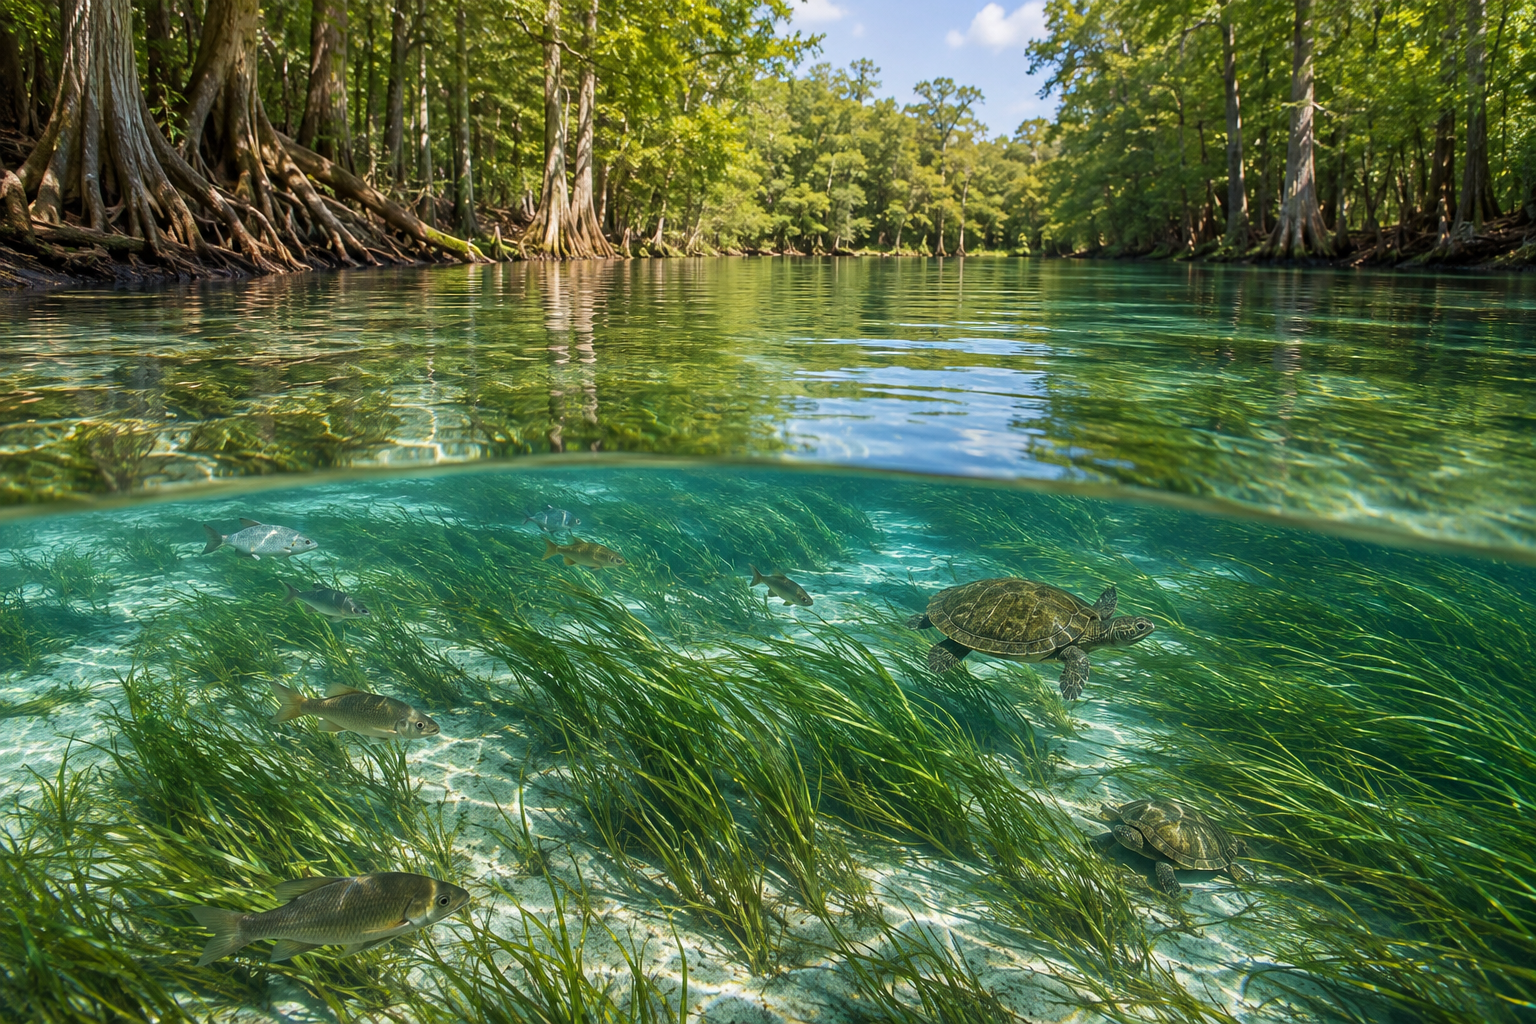
\includegraphics[width=0.6\linewidth]{images/book3/ai/b3-26-clear-spring.png}

{\small Un manantial calizo: una capa de \omterm{def:b1:ecosystem-organization:trophic}{productores} de cintas acuáticas y
algas a plena luz y, por encima, los \omterm{def:b1:ecosystem-organization:trophic}{consumidores} para los que se trazó el
primer balance energético ecológico.}
\end{omfigure}

\section{El flujo de energía}

\begin{definition}[Productividad]\label{def:b1:ecosystem-organization:productivity}
\index{productividad primaria}\index{productividad primaria bruta}\index{productividad primaria neta}
La \emph{productividad primaria bruta} (PPB) de un \omterm{def:b1:ecosystem-organization:ecosystem}{ecosistema} es la
velocidad a la que sus \omterm{def:b1:ecosystem-organization:trophic}{productores} fijan energía por fotosíntesis, por
unidad de superficie y de tiempo (\unit{kJ.m^{-2}.yr^{-1}}, o gramos de
carbono o de materia seca); la \emph{productividad primaria neta} (PPN) es
lo que queda tras la respiración de los propios \omterm{def:b1:ecosystem-organization:trophic}{productores} --- la materia
orgánica realmente puesta a disposición del resto del sistema. La
\emph{productividad secundaria} es la velocidad a la que los \omterm{def:b1:ecosystem-organization:trophic}{consumidores}
construyen su propia biomasa con lo que comen. La \emph{biomasa} es la
existencia presente, la masa que hay en un momento dado; la productividad es
un flujo y la biomasa una reserva, y el cociente de ambas es el tiempo de
renovación.
\end{definition}

\begin{theorem}[La regla del diez por ciento]\label{thm:b1:ecosystem-organization:lindeman}
\index{eficiencia trófica}
De la energía que entra en un \omterm{def:b1:ecosystem-organization:trophic}{nivel trófico} como alimento, solo una décima
parte aproximadamente --- entre el \qty{5}{} y el \qty{20}{\%} --- llega al
nivel siguiente como alimento suyo. El resto no se come, no se asimila (sale
como heces) o lo respira el propio nivel. La energía disponible cae por
tanto diez veces por nivel, que es la razón de que las \omterm{def:b1:ecosystem-organization:foodweb}{cadenas alimentarias}
rara vez superen los cuatro o cinco eslabones, y de que la biomasa y los
efectivos de los depredadores de arriba sean pequeños.
\end{theorem}
\begin{proof}[Demostración parcial]
La energía asimilada por un nivel es lo que come menos lo que excreta; de
ella, la respiración se lleva lo que el nivel gasta en vivir
(\cref{ch:b1:organism-environment}), y solo el resto --- su crecimiento y su
reproducción --- queda disponible para ser comido. Cada una de las tres
fracciones (comida, asimilada, convertida en biomasa) está muy por debajo de
uno: para un herbívoro de un prado se come alrededor del \qty{20}{\%} del
crecimiento vegetal, se asimila el \qty{50}{\%} de eso y se convierte en
carne el \qty{10}{\%} de eso, lo que da el \qty{1}{\%}; para un carnívoro,
que come y asimila una parte mayor de su presa, alrededor del \qty{10}{\%}.
La regla es una regularidad observada, no una ley; su valor es el que dan
las medidas.
\end{proof}
\begin{proof}[Evidencia]
Lindeman (1942) midió, en un lago pequeño, la energía fijada por el plancton
y la energía retenida y respirada en cada nivel por encima de él, y halló
que cada nivel pasaba alrededor de una décima parte. Odum (1957) trazó el
balance completo de un manantial de Florida: de \qty{1.7e6}{kcal} por metro
cuadrado y año de luz solar, los \omterm{def:b1:ecosystem-organization:trophic}{productores} fijaron \num{20800} (bruto),
respiraron \num{12000} y dejaron \num{8800} netos; los herbívoros tomaron
\num{3400} y pasaron \num{380} a los carnívoros; los carnívoros pasaron
\num{20} a los carnívoros de arriba. Las eficiencias fueron del
\qty{1.2}{\%}, el \qty{16}{\%}, el \qty{11}{\%} y el \qty{5}{\%} --- la
regla del diez por ciento con un factor de dos en cada paso.
\end{proof}

\begin{omfigure}
\begin{tikzpicture}[font=\footnotesize, >=Stealth, line cap=round]
  % energy pyramid: widths proportional to log-ish scale of energy
  \fill[omExo!45] (-4.4,0) rectangle (4.4,0.9); \node at (0,0.45) {productores: neto \num{8800} kcal\,m$^{-2}$\,yr$^{-1}$ (bruto \num{20800})};
  \fill[omProp!45] (-2.9,1.1) rectangle (2.9,2.0); \node at (0,1.55) {herbívoros: \num{3400} tomadas, \num{1500} asimiladas};
  \fill[omThm!45] (-1.5,2.2) rectangle (1.5,3.1); \node at (0,2.65) {carnívoros: \num{380}};
  \fill[omDef!45] (-0.5,3.3) rectangle (0.5,4.2); \node[anchor=south] at (0,4.25) {carnívoros de arriba: \num{20}};
  \node[anchor=east, align=right] at (-4.6,0.45) {luz solar:\\ \num{1700000}};
  \node[anchor=east, align=right, gray] at (-3.1,1.55) {\qty{16}{\%}};
  \node[anchor=east, align=right, gray] at (-1.7,2.65) {\qty{11}{\%}};
  \node[anchor=east, align=right, gray] at (-0.7,3.75) {\qty{5}{\%}};
  \draw[->, thick, gray] (4.6,0.45) -- (5.4,0.45) node[right, align=left] {respiración y\\ descomponedores: calor};
  \draw[->, thick, gray] (3.1,1.55) -- (5.4,1.55); \draw[->, thick, gray] (1.7,2.65) -- (5.4,2.65); \draw[->, thick, gray] (0.7,3.75) -- (5.4,3.75);
\end{tikzpicture}

{\small Balance energético de un manantial (kilocalorías por metro cuadrado
y año). Cada nivel pasa al siguiente una décima parte aproximada de lo que
recibe; el resto sale como calor por la respiración, y en su mayor parte a
través de los \omterm{def:b1:ecosystem-organization:trophic}{descomponedores}.}
\end{omfigure}

\begin{proposition}[Pirámides]\label{prop:b1:ecosystem-organization:pyramids}
\index{pirámide ecológica}
Apilar los \omterm{def:b1:ecosystem-organization:trophic}{niveles tróficos} da una \emph{pirámide}. Una pirámide de
\emph{energía} (flujo por nivel) siempre está derecha: cada nivel solo puede
pasar menos de lo que recibió. Una pirámide de \emph{biomasa} (existencia
presente) suele estar derecha, pero puede estar invertida: en mar abierto el
fitoplancton, comido tan deprisa como crece, pesa en un momento dado menos
que el zooplancton que vive de él, porque se renueva en días mientras que
los animales duran meses. Una pirámide de \emph{efectivos} puede tener
cualquier forma: un solo roble alimenta a miles de orugas. La energía es la
medida honrada.
\end{proposition}

\begin{method}[Elaboración de un balance energético]\label{met:b1:ecosystem-organization:budget}
\begin{enumerate}
  \item Mídase la PPB: por intercambio gaseoso (oxígeno liberado o
        $\mathrm{CO_2}$ captado por una parcela o por una botella a la luz y
        a oscuras: la luz menos la oscuridad da la bruta, y la luz sola da
        la neta), o por cosecha (biomasa ganada al año más lo que fue comido
        y desprendido).
  \item Mídanse, para cada nivel de \omterm{def:b1:ecosystem-organization:trophic}{consumidores}, la ingesta (lo que come),
        la asimilación (ingesta menos heces), la respiración (su consumo de
        oxígeno) y la producción (crecimiento más descendencia $=$
        asimilación menos respiración).
  \item \omterm{thm:b1:ecosystem-organization:lindeman}{Eficiencia trófica} entre niveles $=$ producción del nivel superior
        $/$ producción del inferior. Compruébese que respiración más
        producción más descomposición de cada nivel suman su asimilación.
  \item Conviértase a unidades comunes (\unit{kJ}, o gramos de carbono a
        unos \qty{40}{kJ/g}) y dibújese la pirámide; la suma de todas las
        respiraciones debería acercarse a la PPB a lo largo de un año en un
        \omterm{def:b1:ecosystem-organization:ecosystem}{ecosistema} estacionario.
\end{enumerate}
\end{method}

\begin{example}[Por qué la cima es delgada]\label{ex:b1:ecosystem-organization:top}
Un kilómetro cuadrado de sabana produce unas \qty{5000}{t} de hierba al año;
los herbívoros pastadores la convierten en \qty{50}{t} de antílopes y
búfalos; los leones, en \qty{2}{t} de león: uno o dos animales. Para
alimentar a un tigre, un bosque debe ser lo bastante grande como para que su
décima parte de una décima de una décima de la luz solar sea un ciervo
entero cada semana: cien kilómetros cuadrados por tigre, que es la razón de
que los grandes carnívoros sean escasos, recorran grandes distancias y
desaparezcan los primeros cuando un \omterm{def:b1:ecosystem-organization:niche}{hábitat} se encoge.
\end{example}

\begin{proposition}[Productividad de los biomas]\label{prop:b1:ecosystem-organization:biomes}
\index{bioma}
La \omterm{def:b1:ecosystem-organization:productivity}{productividad primaria neta} por unidad de superficie la fijan la luz, la
temperatura, el agua y los nutrientes: selva tropical lluviosa,
\qtyrange{2000}{3500}{} g de materia seca por metro cuadrado y año; bosque
templado y tierras de cultivo, \qtyrange{600}{1500}{}; praderas,
\qtyrange{200}{1500}{}; tundra y desierto, por debajo de \qty{200}{}; mar
abierto, unos \qty{125}{} (luz abundante, nutrientes escasos); costas de
afloramiento y arrecifes, \qtyrange{500}{2500}{}. El océano, dos tercios del
planeta, aporta alrededor de la mitad de la producción mundial; los bosques,
una décima parte de las tierras emergidas, aportan un tercio de la de estas.
Donde el agua y los nutrientes son amplios, la productividad sigue a la luz
y al calor; donde no lo son, los sigue a ellos.
\end{proposition}

\begin{omfigure}
\begin{tikzpicture}
\begin{axis}[
  xbar, bar width=8pt,
  width=0.84\linewidth, height=6.6cm,
  axis x line=bottom, axis y line=left,
  xmin=0, xmax=2600, xlabel={productividad primaria neta (\unit{g.m^{-2}.yr^{-1}}, materia seca)},
  xlabel style={font=\small, at={(axis description cs:0.5,-0.12)}, anchor=north},
  symbolic y coords={desierto, mar abierto, tundra, pradera templada, tierras de cultivo, bosque templado, estuarios y arrecifes, selva tropical},
  ytick=data, tick label style={font=\small},
  enlarge y limits=0.08, xtick={0,500,1000,1500,2000,2500},
  nodes near coords, nodes near coords style={font=\scriptsize, anchor=west},
]
\addplot[fill=omExo!45, draw=omExo] coordinates {(90,desierto) (125,mar abierto) (140,tundra) (600,pradera templada) (650,tierras de cultivo) (1200,bosque templado) (1800,estuarios y arrecifes) (2200,selva tropical)};
\end{axis}
\end{tikzpicture}

{\small \omterm{def:b1:ecosystem-organization:productivity}{Productividad primaria neta} media de los principales biomas. Un
intervalo de veinte veces, fijado por el agua, el calor, la luz y los
nutrientes.}
\end{omfigure}

\begin{omfigure}
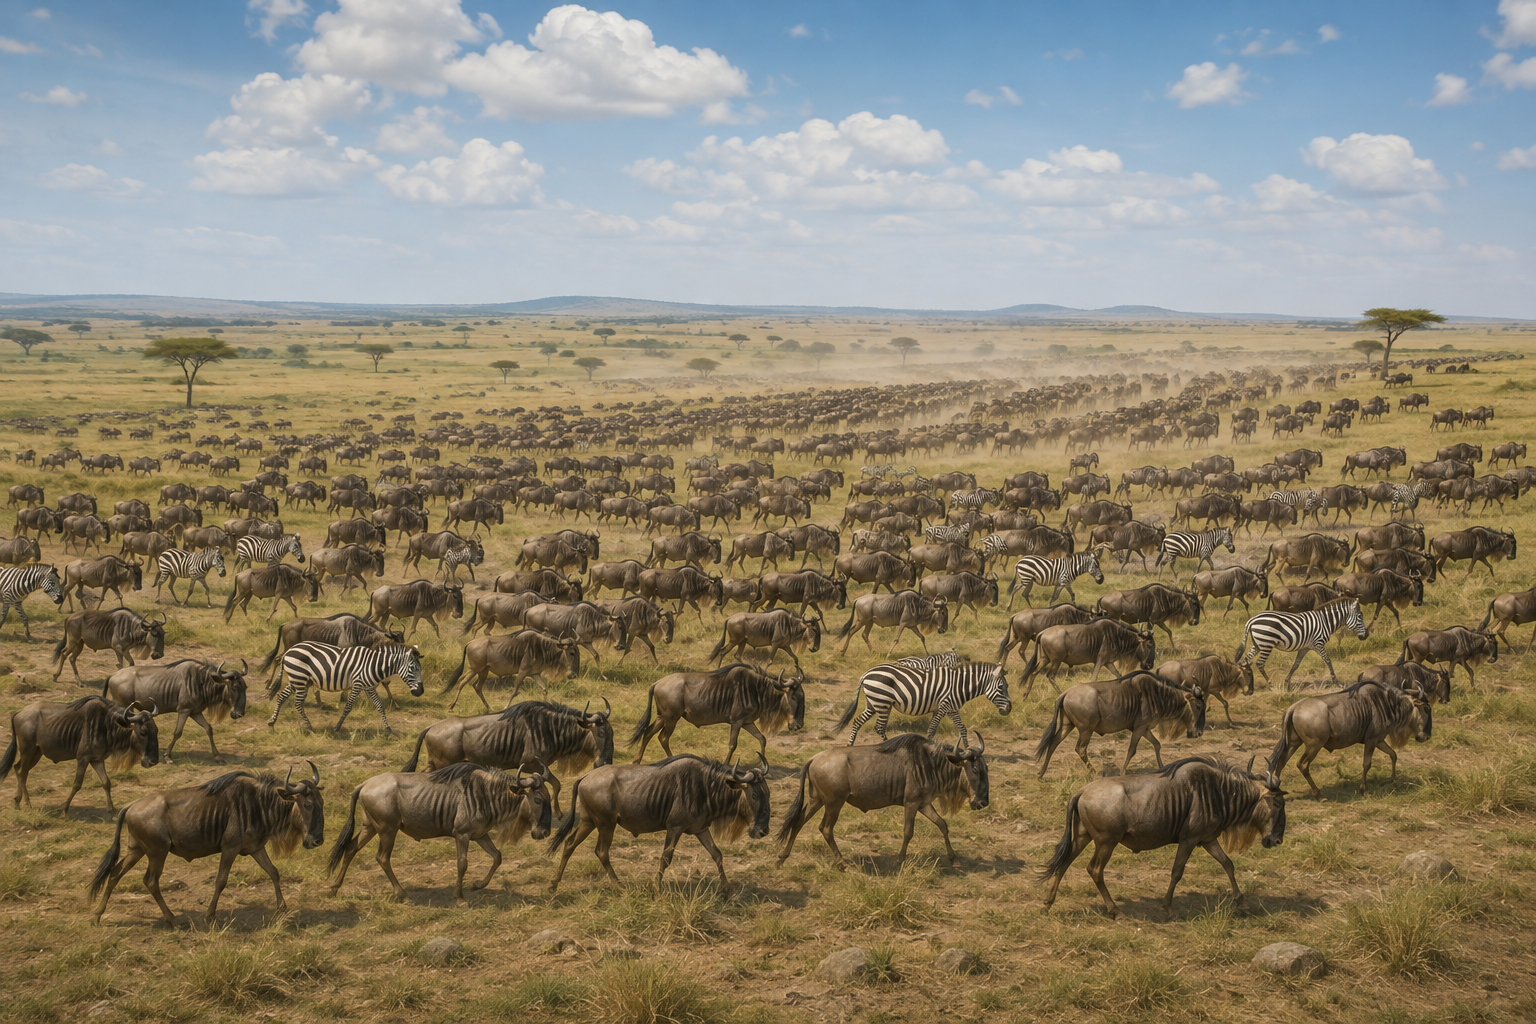
\includegraphics[width=0.6\linewidth]{images/book3/ai/b3-26-wildebeest-migration.png}

{\small Herbívoros pastadores en una sabana: un nivel de \omterm{def:b1:ecosystem-organization:trophic}{consumidores}
primarios de un millón de animales, que siguen a las lluvias que fijan la
productividad de la hierba y llevan una décima parte de su energía a los
depredadores que van tras ellos.}
\end{omfigure}

\section{Contar la diversidad}

\begin{definition}[Riqueza de especies, índice de diversidad]\label{def:b1:ecosystem-organization:diversity}
\index{riqueza de especies}\index{índice de Shannon}
La \emph{riqueza de especies} $S$ de una \omterm{def:b1:ecosystem-organization:ecosystem}{comunidad} es el número de especies
que hay en ella. La riqueza por sí sola ignora la abundancia: un bosque con
cien robles y un ejemplar de cada uno de otros nueve árboles es menos diverso
que otro con diez de cada uno. El \emph{índice de Shannon}
\[
H = -\sum_{i=1}^{S} p_i \ln p_i ,
\]
donde $p_i$ es la fracción de individuos que pertenecen a la especie $i$,
sube tanto con la riqueza como con la \emph{equitatividad}; vale $\ln S$
cuando todas las especies son igual de abundantes y es casi nulo cuando una
domina. La \emph{equitatividad} es $H/\ln S$. La diversidad crece en general
de los polos a los trópicos, con la superficie, con el tiempo transcurrido
desde la última perturbación y con la productividad del lugar hasta cierto
punto.
\end{definition}

\begin{method}[Muestreo de una comunidad]\label{met:b1:ecosystem-organization:sampling}
\begin{enumerate}
  \item Muéstrese con un método adecuado a los \omterm{def:b1:organism-environment:organism}{organismos} (cuadrados, redes,
        trampas, transectos) y regístrese el número de individuos de cada
        especie.
  \item Represéntese el número de especies halladas frente al número de
        muestras (o de individuos): la curva sube de golpe y después se
        aplana; donde se aplana, la riqueza está casi completa. Compárense
        \omterm{def:b1:ecosystem-organization:ecosystem}{comunidades} solo con igual esfuerzo de muestreo.
  \item Calcúlense $H$ y la equitatividad; compárense con el diagrama de
        rango--abundancia (especies ordenadas por abundancia, en escala
        logarítmica), cuya pendiente muestra la dominancia.
  \item Interprétese: una equitatividad baja apunta a una especie dominante
        o a un estrés; una caída de $H$ con el tiempo apunta a un cambio en
        el \omterm{def:b1:ecosystem-organization:ecosystem}{biotopo}.
\end{enumerate}
\end{method}

\begin{example}[Dos bosques]\label{ex:b1:ecosystem-organization:twowoods}
Bosque A: 100 robles y un ejemplar de cada uno de otros nueve árboles;
$H = -(0.917\ln
0.917 + 9\times 0.0092\ln 0.0092) = 0.08 + 0.39 = 0.47$,
equitatividad $0.47/2.30 = 0.20$. Bosque B: diez de cada una de esas mismas
diez especies; $H =
\ln 10 = 2.30$, equitatividad 1. La misma riqueza, cinco
veces la diversidad.
\end{example}

\section{Ejercicios}

\begin{exercise}[$\star$]\label{exo:b1:ecosystem-organization:1}
Defínanse \omterm{def:b1:ecosystem-organization:ecosystem}{ecosistema}, \omterm{def:b1:ecosystem-organization:ecosystem}{comunidad} y \omterm{def:b1:ecosystem-organization:ecosystem}{biotopo}, con el ejemplo de una charca.
\end{exercise}

\begin{exercise}[$\star$]\label{exo:b1:ecosystem-organization:2}
Distínganse \omterm{def:b1:ecosystem-organization:niche}{hábitat} de \omterm{def:b1:ecosystem-organization:niche}{nicho}, y \omterm{def:b1:ecosystem-organization:niche}{nicho} fundamental de \omterm{def:b1:ecosystem-organization:niche}{nicho} realizado.
\end{exercise}

\begin{exercise}[$\star$]\label{exo:b1:ecosystem-organization:3}
A partir de la pirámide energética del manantial, calcúlense la eficiencia
de la luz solar a la producción bruta y la fracción de la producción neta
que se llevaron los herbívoros.
\end{exercise}

\begin{exercise}[$\star$]\label{exo:b1:ecosystem-organization:4}
Nómbrense los cuatro grupos tróficos y dígase cuál de ellos cierra el ciclo
de la materia.
\end{exercise}

\begin{exercise}[$\star\star$]\label{exo:b1:ecosystem-organization:5}
La PPN de un prado es de \qty{800}{g.m^{-2}.yr^{-1}} (\qty{17}{kJ/g}). Los
conejos se comen el \qty{15}{\%}, asimilan el \qty{50}{\%} de lo que comen y
convierten en conejo el \qty{5}{\%} de lo que asimilan. Calcúlense la
producción de conejo por hectárea y la \omterm{thm:b1:ecosystem-organization:lindeman}{eficiencia trófica} de la PPN al
conejo.
\end{exercise}

\begin{exercise}[$\star\star$]\label{exo:b1:ecosystem-organization:6}
Explíquese por qué una pirámide de biomasa puede estar invertida en el mar y
una pirámide de energía nunca lo está.
\end{exercise}

\begin{exercise}[$\star\star$]\label{exo:b1:ecosystem-organization:7}
Calcúlense el \omterm{def:b1:ecosystem-organization:diversity}{índice de Shannon} y la equitatividad de una muestra de 50 A,
30 B, 15 C y 5 D. Compárense con cuatro especies con 25 cada una.
\end{exercise}

\begin{exercise}[$\star\star$]\label{exo:b1:ecosystem-organization:8}
En un experimento de botellas clara y oscura, el oxígeno de la botella clara
sube \qty{3}{mg/L} en un día y el de la botella oscura baja \qty{1}{mg/L}.
Calcúlense las productividades bruta y neta del agua en miligramos de
oxígeno por litro y día, y en gramos de carbono (\qty{1}{g} de
$\mathrm{O_2}$ $\approx$ \qty{0.375}{g} de C).
\end{exercise}

\begin{exercise}[$\star\star$]\label{exo:b1:ecosystem-organization:9}
¿Por qué no hay \omterm{def:b1:ecosystem-organization:foodweb}{cadenas alimentarias} de diez eslabones, y por qué las islas
y los desiertos tienen cadenas más cortas que los bosques?
\end{exercise}

\begin{exercise}[$\star\star\star$]\label{exo:b1:ecosystem-organization:10}
Un ser humano puede comer el grano directamente o dárselo al ganado. Con una
\omterm{thm:b1:ecosystem-organization:lindeman}{eficiencia trófica} del \qty{10}{\%} para el ganado, calcúlese la superficie
necesaria para alimentar a una persona con carne de vacuno frente a con
grano, si el campo rinde \qty{6}{t} de grano por hectárea y una persona
necesita \qty{1}{t} al año. ¿Qué dice esto sobre el \omterm{def:b1:ecosystem-organization:trophic}{nivel trófico} humano y
la \omterm{thm:b1:populations:logistic}{capacidad de carga} del planeta?
\end{exercise}

\begin{exercise}[$\star\star\star$]\label{exo:b1:ecosystem-organization:11}
El mar abierto tiene una PPN baja por metro cuadrado pero la mitad de la
producción mundial. Concíliense ambas cosas, y explíquese por qué sus
pesquerías se concentran en un pequeño porcentaje de su superficie.
\end{exercise}

\begin{exercise}[$\star\star\star$]\label{exo:b1:ecosystem-organization:12}
``Un \omterm{def:b1:ecosystem-organization:ecosystem}{ecosistema} es una máquina para convertir luz solar en calor, con la
vida como subproducto.'' Discútase en un párrafo: flujo de energía frente a
ciclo de la materia, qué hacen los \omterm{def:b1:ecosystem-organization:trophic}{descomponedores} y qué deja fuera la
frase.
\end{exercise}

\section{Problema: el balance de un manantial}

\begin{problem}[{Problema de fin de semana --- el manantial de Odum
elaborado nivel a nivel: de la luz a la hierba, de la hierba al caracol, del
caracol al pez, del pez a la garza, con la respiración y los
descomponedores, hasta llegar a las eficiencias tróficas de cada nivel}]
\label{pb:b1:ecosystem-organization:1}
Un manantial recibe \qty{1.7e6}{kcal} de luz solar por metro cuadrado y año.
Sus \omterm{def:b1:ecosystem-organization:trophic}{productores} fijan \qty{20800}{kcal} (bruto) y respiran \qty{12000}{}.
Los herbívoros comen \qty{3400}{kcal} de materia vegetal, de las cuales
asimilan \qty{1500}{}, respiran \qty{1100}{} y convierten el resto en
crecimiento y descendencia. Los carnívoros comen \qty{380}{kcal}, respiran
\qty{300}{} y producen el resto; los carnívoros de arriba comen
\qty{20}{kcal}, respiran \qty{14}{} y producen \qty{6}{}. Todo lo que no se
come ni se respira va a los \omterm{def:b1:ecosystem-organization:trophic}{descomponedores}, que lo respiran. Tómense
\qty{1}{kcal} $= \qty{4.18}{kJ}$ y \qty{10}{kcal} por gramo de biomasa
seca.

\medskip
\noindent\textbf{Parte I --- Los \omterm{def:b1:ecosystem-organization:trophic}{productores}.}
\begin{enumerate}
  \item Calcúlese la \omterm{def:b1:ecosystem-organization:productivity}{productividad primaria neta}.
  \item Calcúlese la eficiencia de la fotosíntesis: producción bruta sobre
        luz solar. Compárese con el \qty{34}{\%} de
        \cref{ch:b1:photosynthesis} y enumérense tres pérdidas que las
        separan.
  \item ¿Qué fracción de la producción bruta respiran los \omterm{def:b1:ecosystem-organization:trophic}{productores}?
  \item ¿Cuánta producción neta se comen los herbívoros, y cuánta va
        directamente a los \omterm{def:b1:ecosystem-organization:trophic}{descomponedores}?
  \item Exprésese la PPN en gramos de materia seca por metro cuadrado y año
        y sitúese el manantial entre los biomas del capítulo.
  \item ¿Cuánta luz solar, por metro cuadrado y año, sale del manantial como
        calor sin haber pasado nunca por un \omterm{def:b1:organism-environment:organism}{organismo} vivo?
\end{enumerate}

\medskip
\noindent\textbf{Parte II --- Los \omterm{def:b1:ecosystem-organization:trophic}{consumidores}.}
\begin{enumerate}[resume]
  \item Calcúlense la producción de los herbívoros y su eficiencia de
        asimilación (asimilado/comido).
  \item Calcúlese la eficiencia de producción de los herbívoros
        (producción/asimilado).
  \item Calcúlese la \omterm{thm:b1:ecosystem-organization:lindeman}{eficiencia trófica} de \omterm{def:b1:ecosystem-organization:trophic}{productores} a herbívoros:
        producción de herbívoros sobre producción primaria neta.
  \item Calcúlense la producción de los carnívoros y la \omterm{thm:b1:ecosystem-organization:lindeman}{eficiencia trófica}
        de herbívoros a carnívoros.
  \item Calcúlese la \omterm{thm:b1:ecosystem-organization:lindeman}{eficiencia trófica} de carnívoros a carnívoros de
        arriba.
  \item ¿Cuánta energía por metro cuadrado y año llega a los propios \omterm{def:b1:body-plans-tissues:tissue}{tejidos}
        del carnívoro de arriba? ¿Qué fracción de la luz solar es eso?
  \item ¿Por qué sube la eficiencia de asimilación de los herbívoros a los
        carnívoros?
\end{enumerate}

\medskip
\noindent\textbf{Parte III --- Los \omterm{def:b1:ecosystem-organization:trophic}{descomponedores} y el balance.}
\begin{enumerate}[resume]
  \item Enumérense todos los flujos hacia los \omterm{def:b1:ecosystem-organization:trophic}{descomponedores} (producción
        neta no comida, heces de los herbívoros y producción de herbívoros
        no comida, y así sucesivamente) y súmense.
  \item Calcúlese la respiración total del \omterm{def:b1:ecosystem-organization:ecosystem}{ecosistema}: \omterm{def:b1:ecosystem-organization:trophic}{productores},
        herbívoros, carnívoros, carnívoros de arriba y \omterm{def:b1:ecosystem-organization:trophic}{descomponedores}.
  \item Compárese con la producción bruta. ¿Qué significa la comparación
        para la biomasa del manantial a lo largo de un año?
  \item ¿Qué fracción de la producción bruta respiran los \omterm{def:b1:ecosystem-organization:trophic}{descomponedores}?
  \item Dibújese la pirámide de energía con la producción de los cuatro
        niveles y anótense las eficiencias.
\end{enumerate}

\medskip
\noindent\textbf{Parte IV --- Existencias, renovación y cambio.}
La biomasa presente es de \qty{800}{g/m^2} de \omterm{def:b1:ecosystem-organization:trophic}{productores}, \qty{40}{g/m^2}
de herbívoros, \qty{10}{g/m^2} de carnívoros y \qty{1.5}{g/m^2} de
carnívoros de arriba.
\begin{enumerate}[resume]
  \item Conviértase cada biomasa a kilocalorías y dibújese la pirámide de
        biomasa. ¿Está derecha?
  \item Calcúlese el tiempo de renovación (biomasa/producción) de cada
        nivel. ¿Cuál se renueva más deprisa, y por qué?
  \item Una garza de \qty{2}{kg} vive de la producción de carnívoros de
        arriba del manantial. ¿Cuántos metros cuadrados necesita?
  \item Se enriquece el manantial con abono y su producción bruta se
        duplica, pero los herbívoros no pueden comer más deprisa. ¿Qué
        ocurre con la producción sobrante, con la respiración de los
        \omterm{def:b1:ecosystem-organization:trophic}{descomponedores} y con el oxígeno del agua de noche?
  \item Se introduce un pez nuevo que come los huevos de los herbívoros y
        reduce a la mitad su producción. Predígase la producción de los
        carnívoros y los efectivos de las garzas, y el destino de las cintas
        acuáticas.
  \item Explíquese por qué retirar los carnívoros de arriba cambiaría las
        cintas acuáticas mucho más que retirar el equivalente energético en
        herbívoros.
  \item Enúnciese el resultado: las \omterm{thm:b1:ecosystem-organization:lindeman}{eficiencias tróficas} de cada una de las
        tres transferencias, la eficiencia de la luz solar a la producción
        bruta y la fracción de la energía del sol que llega a los carnívoros
        de arriba.
\end{enumerate}
\end{problem}
